\documentclass{beamer}
\mode<presentation>
\usepackage{amsmath,amssymb,mathtools}
\usepackage{textcomp}
\usepackage{gensymb}
\usepackage{adjustbox}
\usepackage{subcaption}
\usepackage{enumitem}
\usepackage{multicol}
\usepackage{listings}
\usepackage{url}
\usepackage{graphicx} % <-- needed for images
\def\UrlBreaks{\do\/\do-}

\usetheme{Boadilla}
\usecolortheme{lily}
\setbeamertemplate{footline}{
  \leavevmode%
  \hbox{%
  \begin{beamercolorbox}[wd=\paperwidth,ht=2ex,dp=1ex,right]{author in head/foot}%
    \insertframenumber{} / \inserttotalframenumber\hspace*{2ex}
  \end{beamercolorbox}}%
  \vskip0pt%
}
\setbeamertemplate{navigation symbols}{}

\lstset{
  frame=single,
  breaklines=true,
  columns=fullflexible,
  basicstyle=\ttfamily\tiny   % tiny font so code fits
}

\numberwithin{equation}{section}

% ---- your macros ----
\providecommand{\nCr}[2]{\,^{#1}C_{#2}}
\providecommand{\nPr}[2]{\,^{#1}P_{#2}}
\providecommand{\mbf}{\mathbf}
\providecommand{\pr}[1]{\ensuremath{\Pr\left(#1\right)}}
\providecommand{\qfunc}[1]{\ensuremath{Q\left(#1\right)}}
\providecommand{\sbrak}[1]{\ensuremath{{}\left[#1\right]}}
\providecommand{\lsbrak}[1]{\ensuremath{{}\left[#1\right.}}
\providecommand{\rsbrak}[1]{\ensuremath{\left.#1\right]}}
\providecommand{\brak}[1]{\ensuremath{\left(#1\right)}}
\providecommand{\lbrak}[1]{\ensuremath{\left(#1\right.}}
\providecommand{\rbrak}[1]{\ensuremath{\left.#1\right)}}
\providecommand{\cbrak}[1]{\ensuremath{\left\{#1\right\}}}
\providecommand{\lcbrak}[1]{\ensuremath{\left\{#1\right.}}
\providecommand{\rcbrak}[1]{\ensuremath{\left.#1\right\}}}
\theoremstyle{remark}
\newtheorem{rem}{Remark}
\newcommand{\sgn}{\mathop{\mathrm{sgn}}}
\providecommand{\abs}[1]{\left\vert#1\right\vert}
\providecommand{\res}[1]{\Res\displaylimits_{#1}}
\providecommand{\norm}[1]{\lVert#1\rVert}
\providecommand{\mtx}[1]{\mathbf{#1}}
\providecommand{\mean}[1]{E\left[ #1 \right]}
\providecommand{\fourier}{\overset{\mathcal{F}}{ \rightleftharpoons}}
\providecommand{\system}{\overset{\mathcal{H}}{ \longleftrightarrow}}
\providecommand{\dec}[2]{\ensuremath{\overset{#1}{\underset{#2}{\gtrless}}}}
\newcommand{\myvec}[1]{\ensuremath{\begin{pmatrix}#1\end{pmatrix}}}
\let\vec\mathbf

\title{Matgeo Presentation - Problem 1.2.10}
\author{ai25btech11004 - jaswanth}

\begin{document}


\frame{\titlepage}
\begin{frame}{Question}
Find the vector joining the points $\Vec{P}$(2,3,0) and $\Vec{Q}$(-1,-2,-4) directed from $\vec{P}$  to $\vec{Q}$.
\end{frame}

\begin{frame}{Solution}
\begin{table}[h!]    
  \centering
  

  \caption{Variables Used}
  \label{}
\end{table}
 \text{The vector joining $\vec{P}$ and $\vec{Q}$ = $\vec{Q}$ - $\vec{P}$}\\
 $\implies$ $\vec{Q}-\vec{P}$ = \myvec{-1\\-2\\-4} - \myvec{2\\3\\0} = \myvec{-3\\-5\\-4} \\
$\implies$ The desired vector is \myvec{-3\\-5\\-4} 
\end{frame}
\begin{frame}{Plot}
   \begin{figure}[h!]
   \centering
   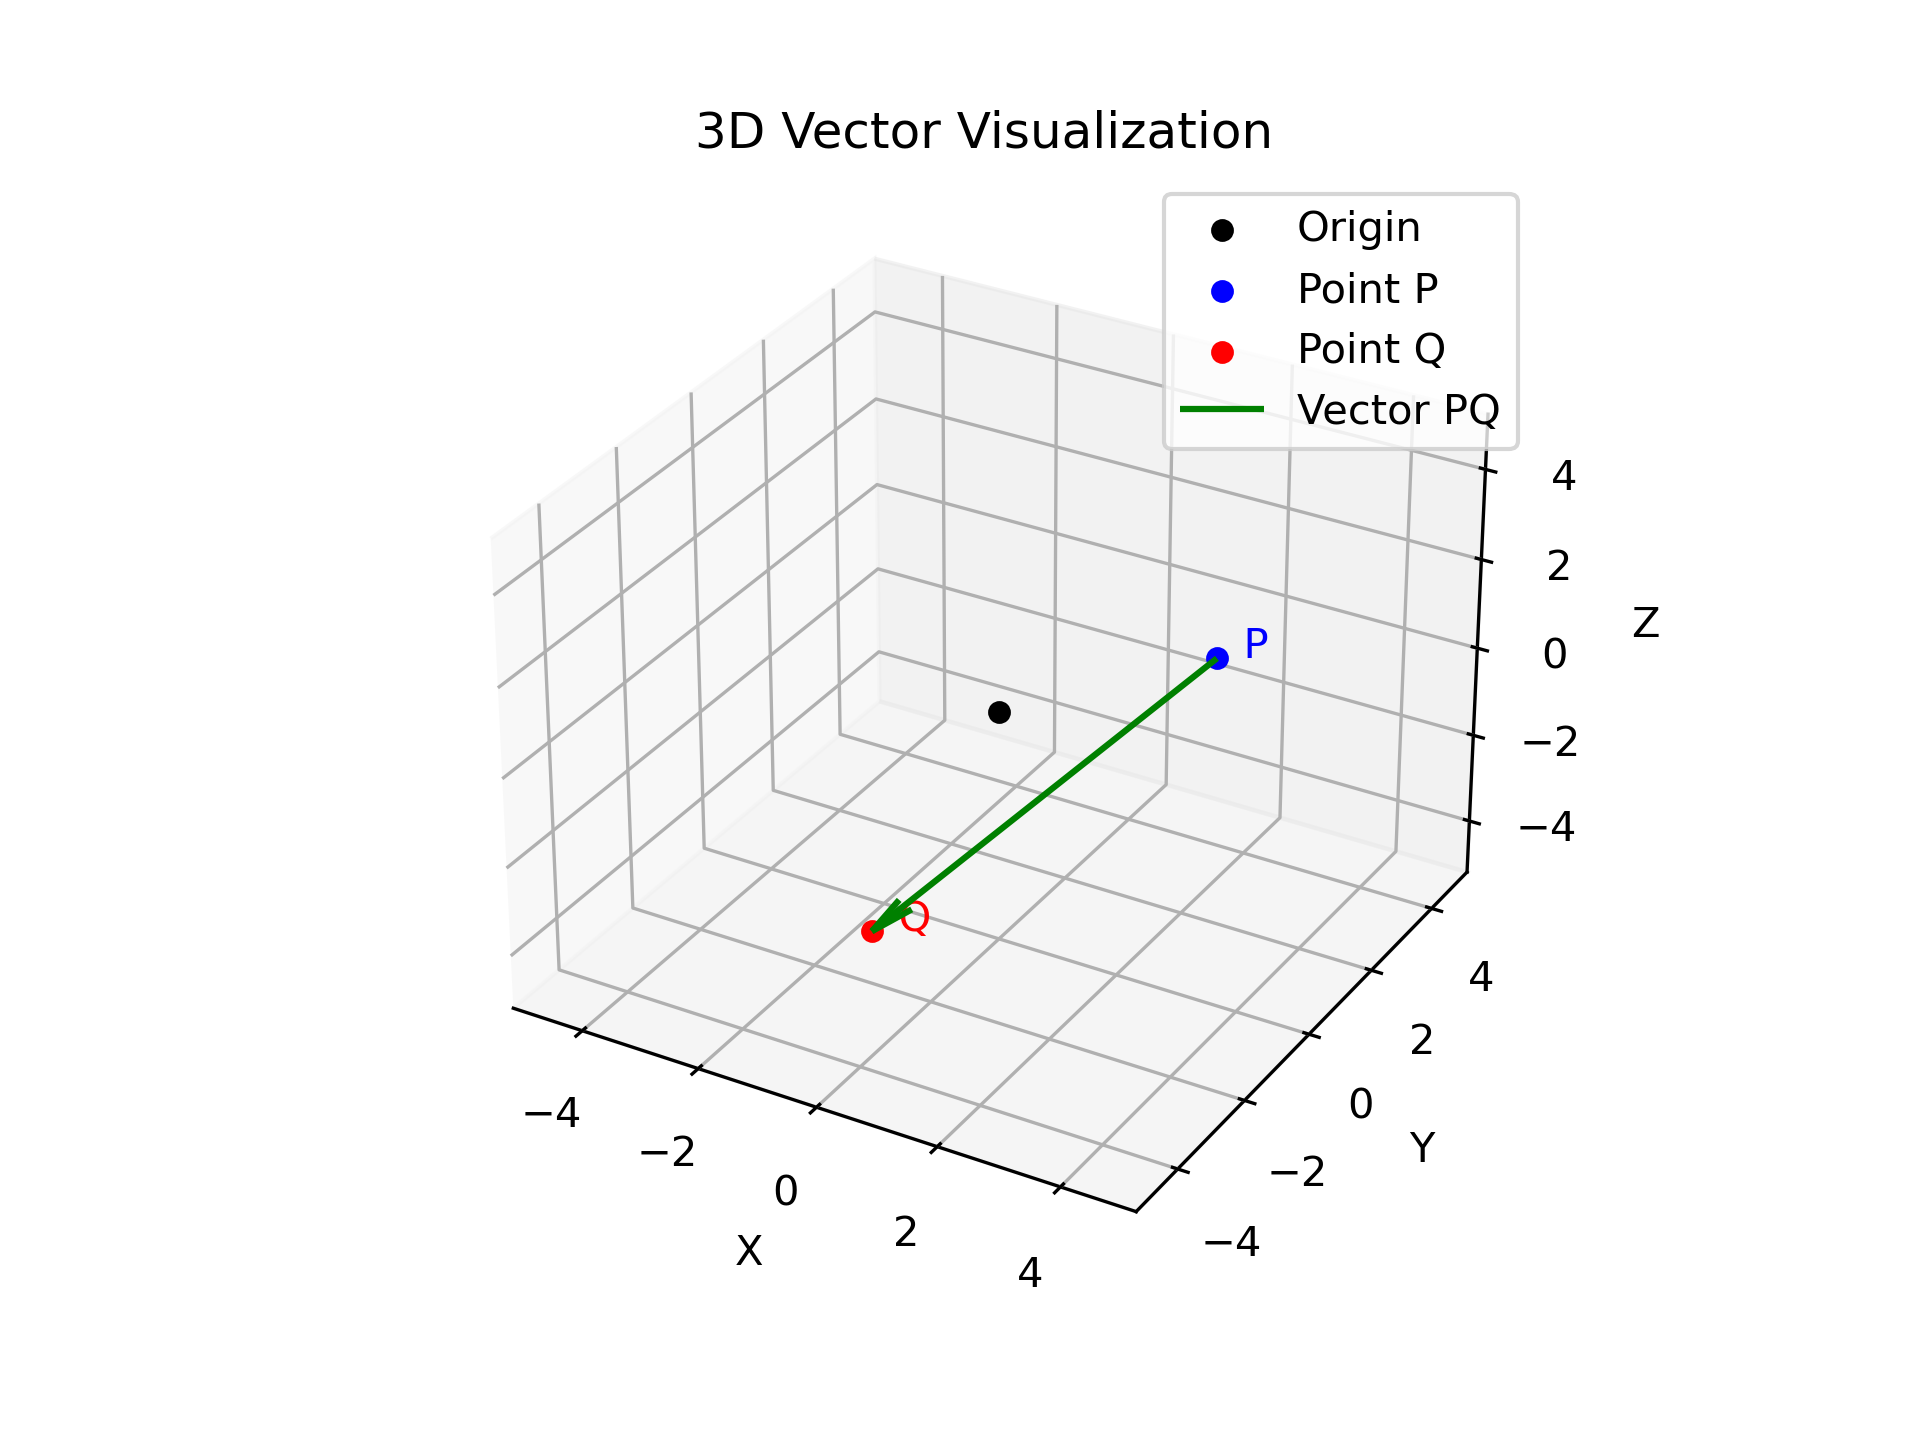
\includegraphics[width=0.8\linewidth]{figs/01.png}
   \caption{}
   \label{}
\end{figure}  
\end{frame}

% --------- CODE APPENDIX ---------
\section*{Appendix: Code}

% C program
\begin{frame}[fragile]{C Code: code.c}
\begin{lstlisting}[language=C]
#include <stdio.h>

int main() {
    FILE *fp;

    // Coordinates of P and Q
    int Px = 2, Py = 3, Pz = 0;
    int Qx = -1, Qy = -2, Qz = -4;

    // Vector from P to Q: Q - P
    int Vx = Qx - Px;
    int Vy = Qy - Py;
    int Vz = Qz - Pz;

    // Open file for writing
    fp = fopen("vector.dat", "w");
    if (fp == NULL) {
        printf("Error opening file!\n");
        return 1;
    }

    // Write vector to file
    fprintf(fp, "Vector from P(%d,%d,%d) to Q(%d,%d,%d):\n", Px, Py, Pz, Qx, Qy, Qz);
    fprintf(fp, "Vector PQ = (%d, %d, %d)\n", Vx, Vy, Vz);

    // Close file
    fclose(fp);

    printf("Vector successfully written to vector.dat\n");
    return 0;
}
\end{lstlisting}
\end{frame}

% Python calling C
\begin{frame}[fragile]{Python: call.py}
\begin{lstlisting}[language=Python]
import subprocess
import os

# Compile the C code
compile_process = subprocess.run(["gcc", "code.c", "-o", "code.out"])

# Check if compilation was successful
if compile_process.returncode == 0:
    print("Compilation successful. Running the program...\n")
    
    # Run the compiled program
    run_process = subprocess.run(["./code.out"])
else:
    print("Compilation failed.")
\end{lstlisting}
\end{frame}

% Python plotting
\begin{frame}[fragile]{Python: plot.py}
\begin{lstlisting}[language=Python]

import numpy as np
import matplotlib.pyplot as plt

# Read vector data from file
with open('vector.dat', 'r') as file:
    lines = file.readlines()

# Extract coordinates from the file
line1 = lines[0]
P_start = line1.split("P(")[1].split(")")[0]
Q_end = line1.split("Q(")[1].split(")")[0]

P = np.array(list(map(int, P_start.split(','))))
Q = np.array(list(map(int, Q_end.split(','))))
PQ = Q - P  # Vector from P to Q

# Set up the 3D plot
fig = plt.figure()
ax = fig.add_subplot(111, projection='3d')

# Plot origin
ax.scatter(0, 0, 0, color='black', label='Origin')

# Plot points
ax.scatter(*P, color='blue', label='Point P')
ax.scatter(*Q, color='red', label='Point Q')

# Plot vector PQ (arrow from P to Q)
ax.quiver(*P, *PQ, color='green', arrow_length_ratio=0.1, label='Vector PQ')

# Annotate points
ax.text(*P, '  P', color='blue')
\end{lstlisting}
\end{frame}

\begin{frame}[fragile]{Python: plot.py}
\begin{lstlisting}[language=Python]
ax.text(*Q, '  Q', color='red')

# Set limits
max_range = np.max(np.abs([P, Q])) + 1
ax.set_xlim([-max_range, max_range])
ax.set_ylim([-max_range, max_range])
ax.set_zlim([-max_range, max_range])

# Labels and legend
ax.set_xlabel('X')
ax.set_ylabel('Y')
ax.set_zlabel('Z')
ax.set_title('3D Vector Visualization')
ax.legend()

# Save the figure as an image (e.g., PNG)
plt.savefig('vector_plot.png', dpi=300)  # Change filename/format if needed

print("Plot saved as vector_plot.png")
\end{lstlisting}
\end{frame}
\end{document}
